%!TEX root = main.tex
\setcounter{chapter}{2}
\setcounter{section}{4}
\setcounter{theorem}{0}
\setcounter{equation}{0}

\lectureheader{161}{Calculus I}{One-sided limits}{\textit{Thomas' Calculus} \thesection}
\begin{definition}
Let $c\in\R$, and let $f$ be a function so that every interval of the form $(c,b)$ also contains points of $\dom(f)$.
We say that $L$ is \textbf{limit of $f(x)$ as $x$ approaches $c$ from the right}, and we write
\begin{equation*}
\lim_{x\to c^+}f(x) = L,
\end{equation*}
provided that for every $\epsilon>0$, there is a $\delta>0$ such that
\begin{equation*}
x\in\dom(f)\text{ and }c< x<c+\delta \implies |f(x)-L|<\epsilon.
\end{equation*}
\end{definition}

\begin{definition}
Let $c\in\R$, and let $f$ be a function so that every interval of the form $(a,c)$ also contains points of $\dom(f)$.
We say that $L$ is \textbf{limit of $f(x)$ as $x$ approaches $c$ from the left}, and we write
\begin{equation*}
\lim_{x\to c^-}f(x) = L,
\end{equation*}
provided that for every $\epsilon>0$, there is a $\delta>0$ such that
\begin{equation*}
x\in\dom(f)\text{ and }c-\delta< x<c \implies |f(x)-L|<\epsilon.
\end{equation*}
\end{definition}
\begin{remark}\,
\begin{itemize}
\item The limit from the right only cares about what is happening to $f(x)$ as $x$ approaches $c$ from the right through $x$-values (other than $c$) in $\dom(f)$.
\item The limit from the left only cares about what is happening to $f(x)$ as $x$ approaches $c$ from the left through $x$-values (other than $c$) in $\dom(f)$.
\end{itemize}
\end{remark}

\newpage

\begin{example}
Evaluate the limits below for the function $f(x) = \sqrt{4-x^2}$.
\begin{figure}[H]
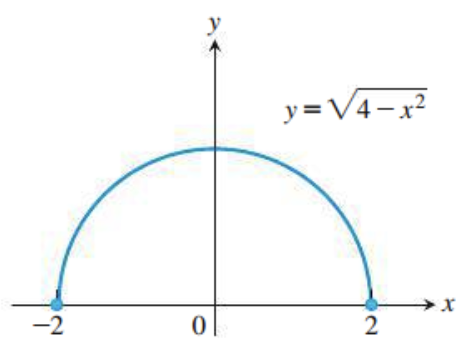
\includegraphics[width=3in]{img/one-sided-ex1}
\end{figure}
\begin{enumerate}
\item $\DS\lim_{x\to 2^-}f(x)$
\vfill
\item $\DS\lim_{x\to 2^+}f(x)$
\vfill
\item If $c\in [-2,2]$, then $\DS\lim_{x\to c}f(x)$
\vfill
\end{enumerate}
\end{example}

\newpage

\begin{theorem}
Let $c\in\R$, and let $f$ be a function so that every interval of the form $(a,c)$ and every interval of the form $(c,b)$ contains points of $\dom(f)$.
Then
\begin{equation*}
\lim_{x\to c}f(x)=L \iff \lim_{x\to c^+}f(x)=L \text{ and } \lim_{x\to c^-}f(x)=L.
\end{equation*}
\end{theorem}

\begin{example}
Use the graph below to evaluate the limits.
\begin{figure}[H]
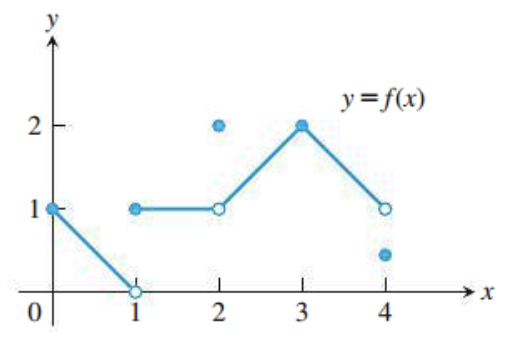
\includegraphics[width=3in]{img/one-sided-ex2}
\end{figure}
\begin{minipage}{3in}
\begin{enumerate}
\item $\DS\lim_{x\to 0^+}f(x)$
\vspace{0.3in}
\item $\DS\lim_{x\to 0}f(x)$
\vspace{0.3in}
\item $\DS\lim_{x\to 1^-}f(x)$
\vspace{0.3in}
\item $\DS\lim_{x\to 1^+}f(x)$
\vspace{0.3in}
\item $\DS\lim_{x\to 1}f(x)$
\vspace{0.3in}
\item $\DS\lim_{x\to 2^-}f(x)$
\vspace{0.3in}
\item $\DS\lim_{x\to 2^+}f(x)$
\vspace{0.3in}
\item $\DS\lim_{x\to 2}f(x)$
\vspace{0.3in}
\end{enumerate}
\end{minipage}
\begin{minipage}{3in}
\begin{enumerate}
\setcounter{enumi}{8}

\vfill
\item $\DS\lim_{x\to 3^-}f(x)$
\vspace{0.3in}
\item $\DS\lim_{x\to 3^+}f(x)$
\vspace{0.3in}
\item $\DS\lim_{x\to 3}f(x)$
\vspace{0.3in}
\item $\DS\lim_{x\to 4^-}f(x)$
\vspace{0.3in}
\item $\DS\lim_{x\to 4}f(x)$
\vspace{2in}
\end{enumerate}
\end{minipage}
\end{example}

\newpage

%\begin{example}
%Prove that $\DS\lim_{x\to 0^+}\sqrt x = 0$.
%\end{example}
%
%
%
%\newpage

\begin{theorem}
\begin{equation*}
\lim_{\theta\to 0}\frac{\sin\theta}{\theta} = 1.
\end{equation*}
\end{theorem}
\begin{flushright}
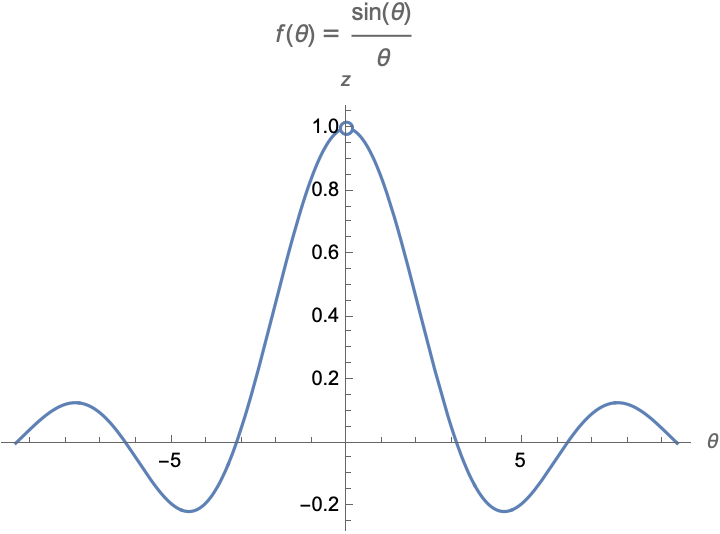
\includegraphics[width=3.5in]{img/one-sided-ex5}
\end{flushright}

\newpage

\begin{example}
Evaluate the limits.
\begin{enumerate}
\item $\DS\lim_{y\to 0}\frac{\cos y -1}{y}$
\vfill
\item $\DS\lim_{x\to 0}\frac{\sin 2x}{5x}$
\vfill
\item $\DS\lim_{x\to 0}\frac{\sin 3x}{\sin 7x}$
\vfill
\item $\DS\lim_{t\to 0}\frac{\tan t\sec 2t}{3t}$
\vfill
\end{enumerate}
\end{example}
